    \subsection[\theta]{Inclinazione orbita}
        \begin{frame}{Orbite 3D}
            \begin{columns}
                \column{.45\textwidth}
                    \begin{block}{Modifiche al codice}
                        \begin{enumerate}
                            \item modifiche ai file di configurazione e alla funzione sistema::leggi()
                            \item aggiunta funzione vettore::angolo() per il calcolo dell'angolo tra due vettori nello spazio
                            \item inserimento del codice seguente nella funzione corpo::evolvidt()
                            \begin{enumerate}[i]
                                \item calcolo dell'angolo ad ogni step rispetto a piano eclittica istantaneo
                                \item raccolta dati in istogramma
                            \end{enumerate}
                        \end{enumerate}
                    \end{block}
                \column{.55\textwidth}
                    %\centering
                    %da sistemare - voglio mettere codice
                    %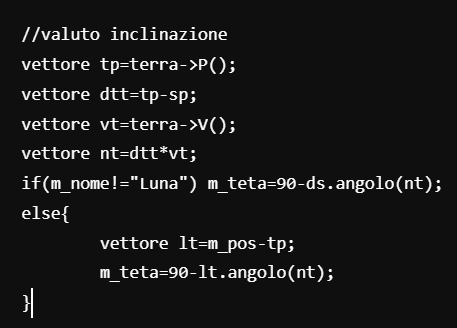
\includegraphics[width=.9\textwidth]{7_incli/code.png}
                    \begin{lstlisting}[language=C++]
//valuto inclinazione 
corpo *terra=cc[3]; 
vettore tp=terra->P(); 
vettore dtt=tp-sp; 
vettore vt=terra->V(); 
vettore nt=dtt*vt; 
if(m_nome!="Luna") 
    m_teta=90-ds.angolo(nt); 
else{ 
    vettore lt=m_pos-tp; 
    m_teta=90-lt.angolo(nt); 
}
\end{lstlisting}
            \end{columns}
        \end{frame}
        
        \begin{frame}{Orbite 3D - stabili nei limiti evidenziati sopra}
            \begin{columns}
                \column{.5\textwidth}
                    \centering        
                    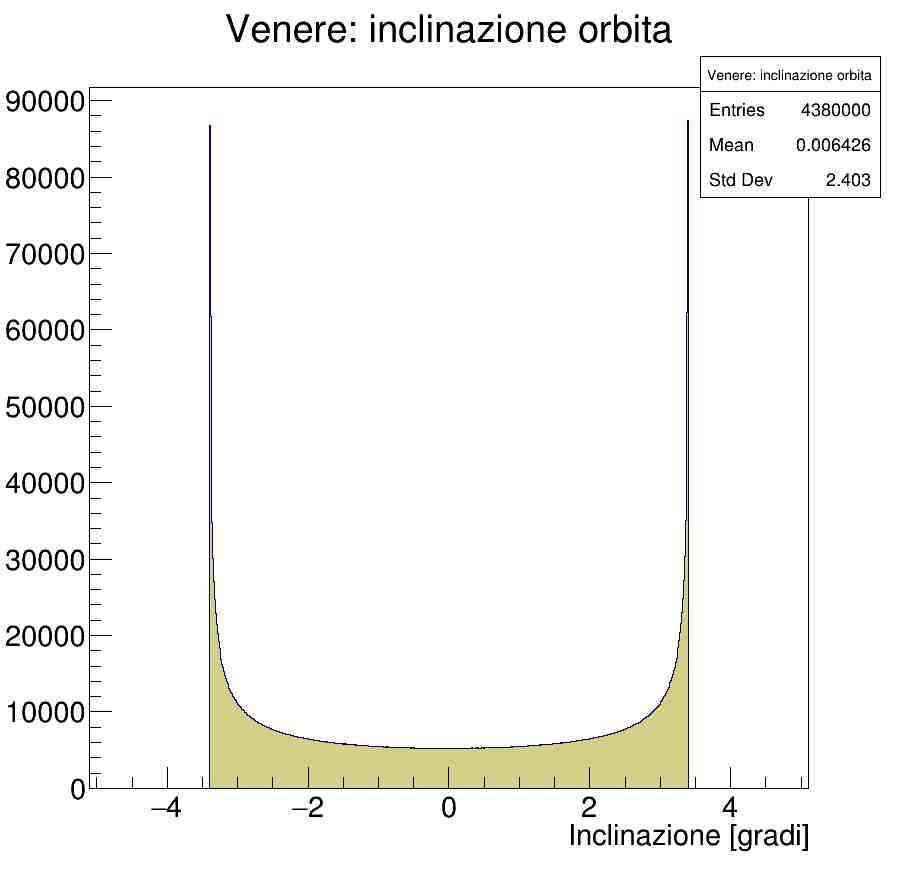
\includegraphics[width=5cm,height=3.75cm]{7_incli/ven_incl_500_3600.jpg}\\
                    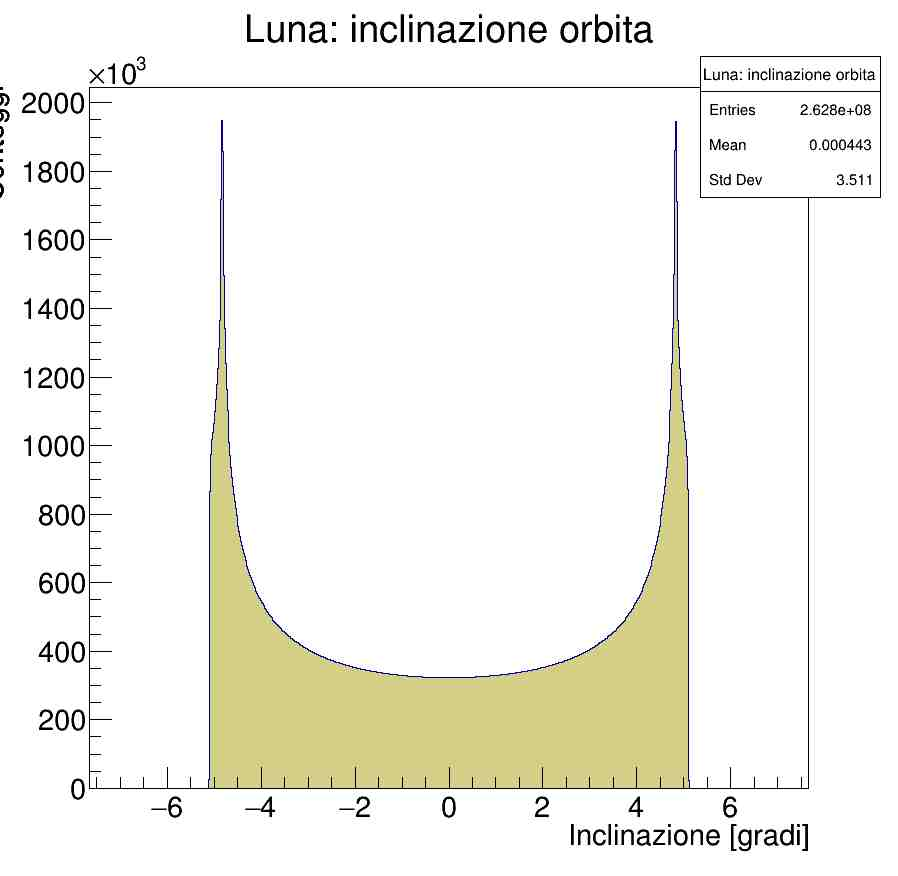
\includegraphics[width=5cm,height=3.75cm]{7_incli/lun_incl_600_60.jpg}
                    \label{cfr::vin}              
                \column{.5\textwidth}
                    \centering        
                    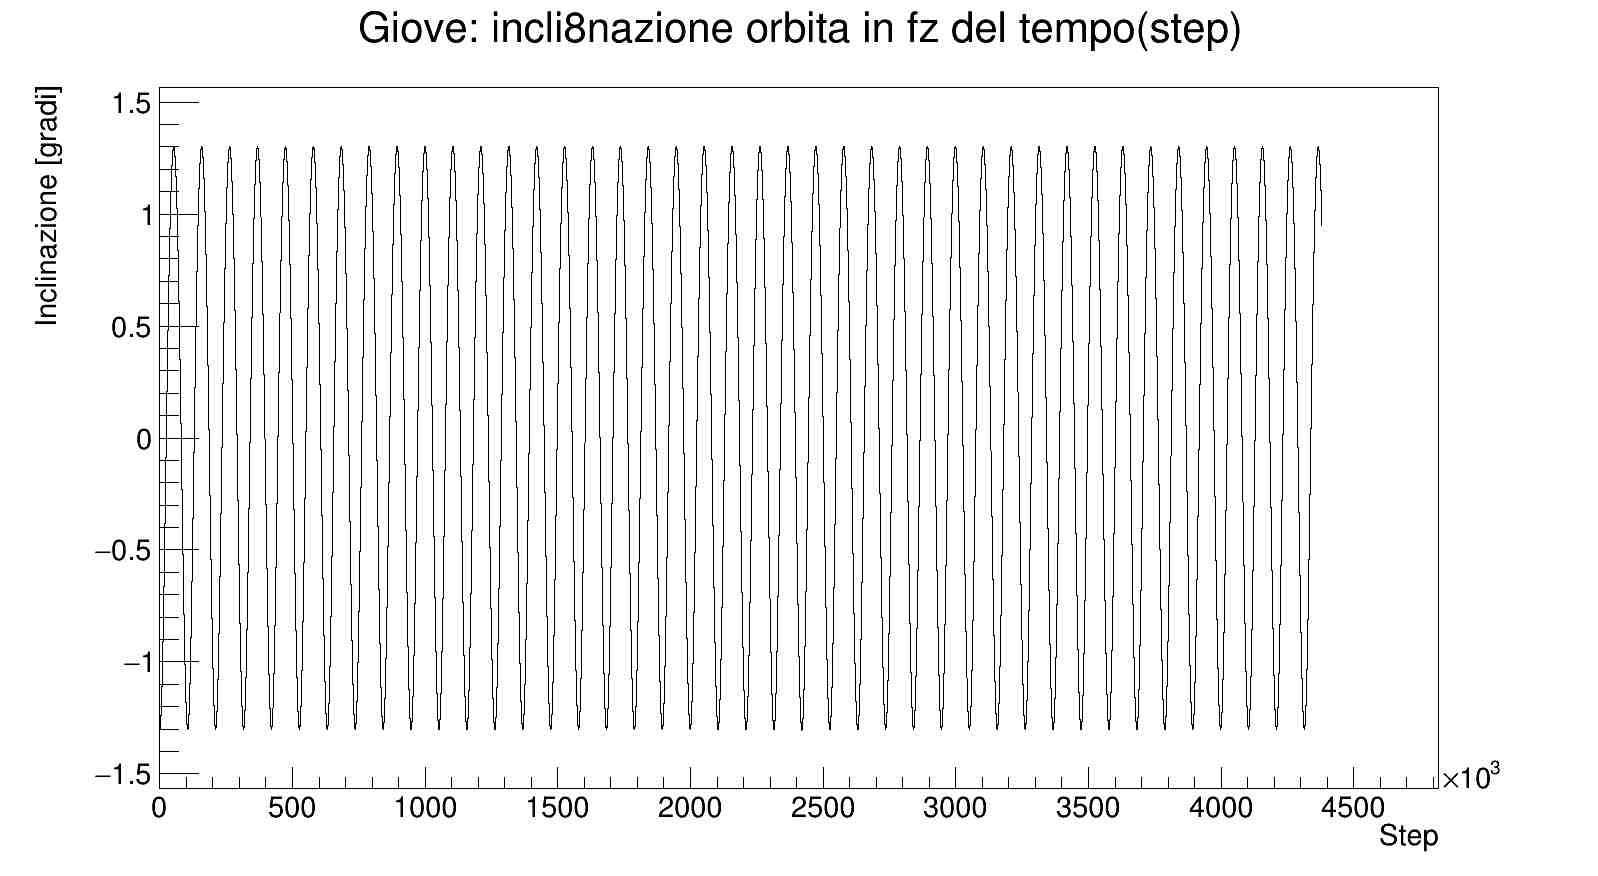
\includegraphics[width=5cm,height=3.75cm]{7_incli/gio_inc_temp_500_3600.jpg}\\
                    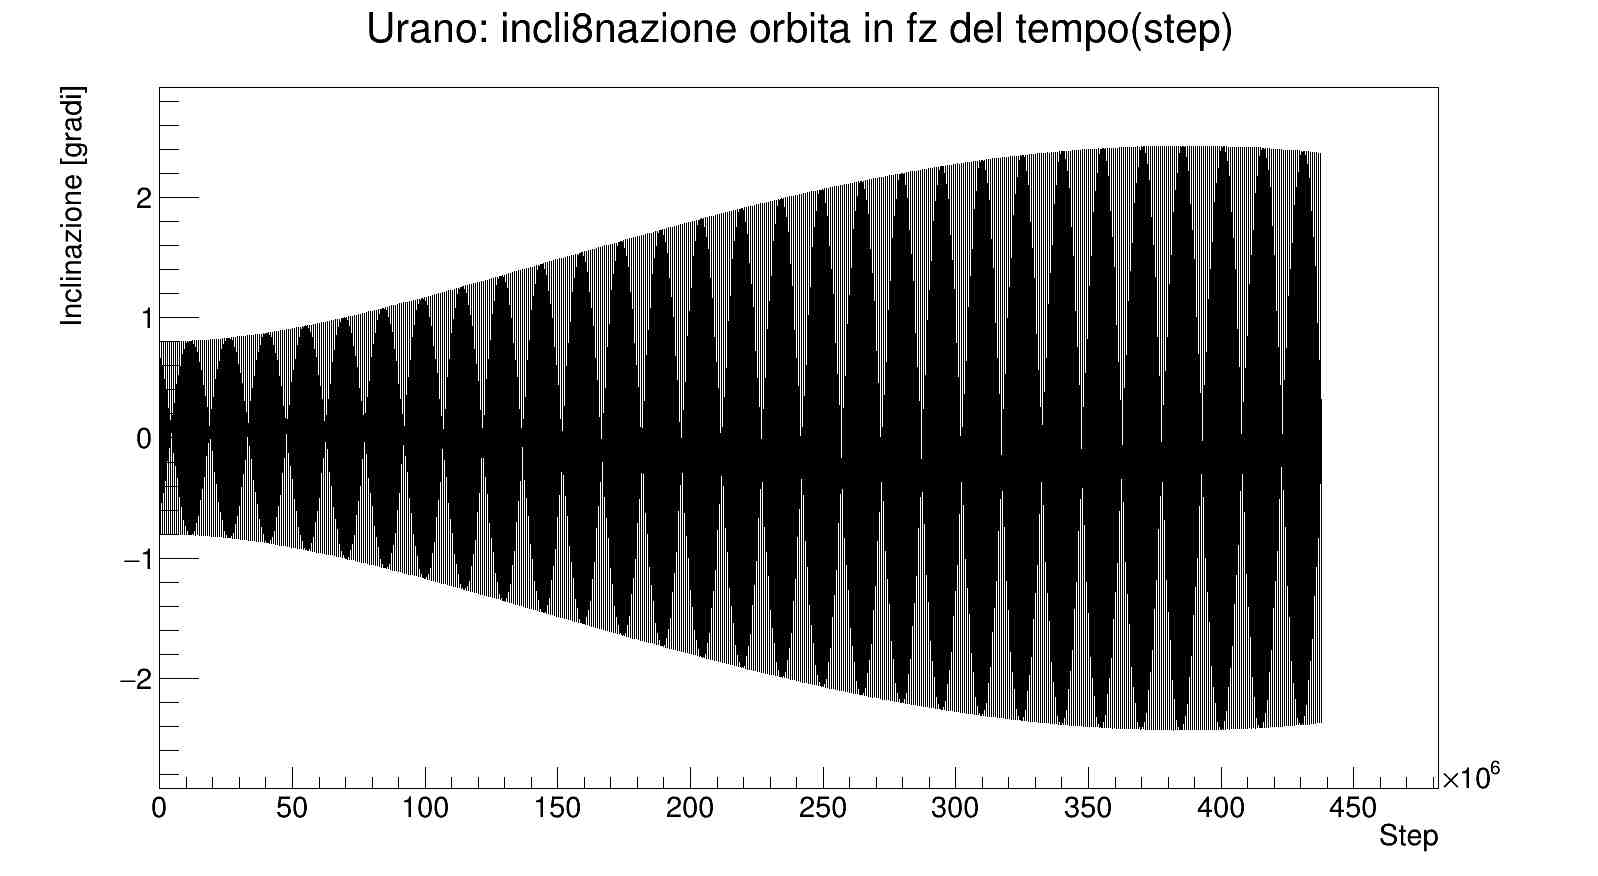
\includegraphics[width=5cm,height=3.75cm]{7_incli/ura_inc_bug_50k_3600.jpg}
                    \label{cfr::sdf}
            \end{columns}
        \end{frame}
        
        \begin{frame}{Grafici con Python}
            \begin{columns}
                \column{.5\textwidth}
                    \centering        
                    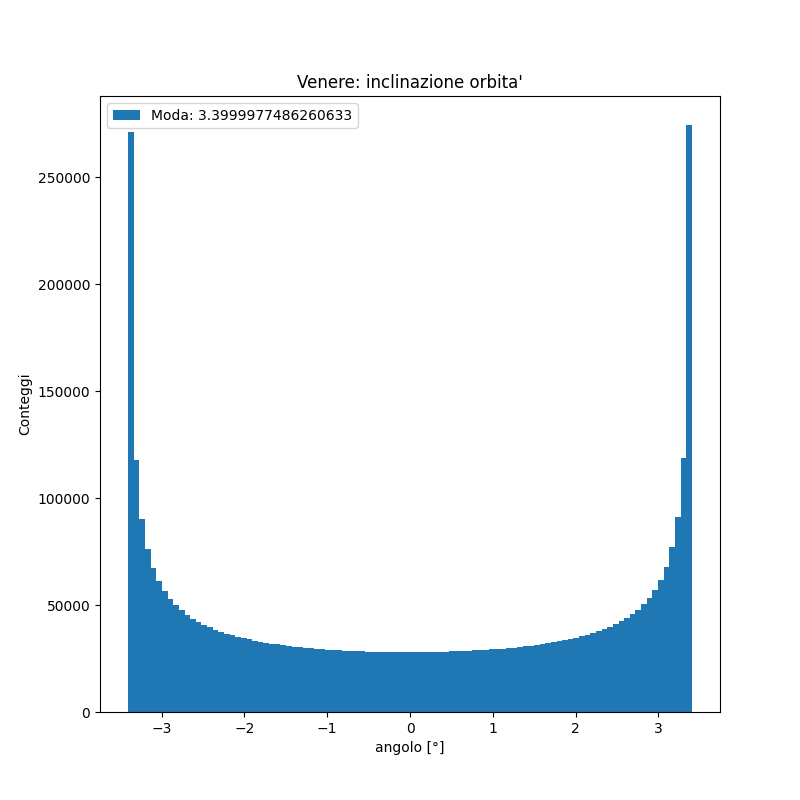
\includegraphics[width=5cm,height=3.75cm]{7_incli/ven_teta.png}\\
                    \label{cfr::in}              
                \column{.5\textwidth}
                    \centering        
                    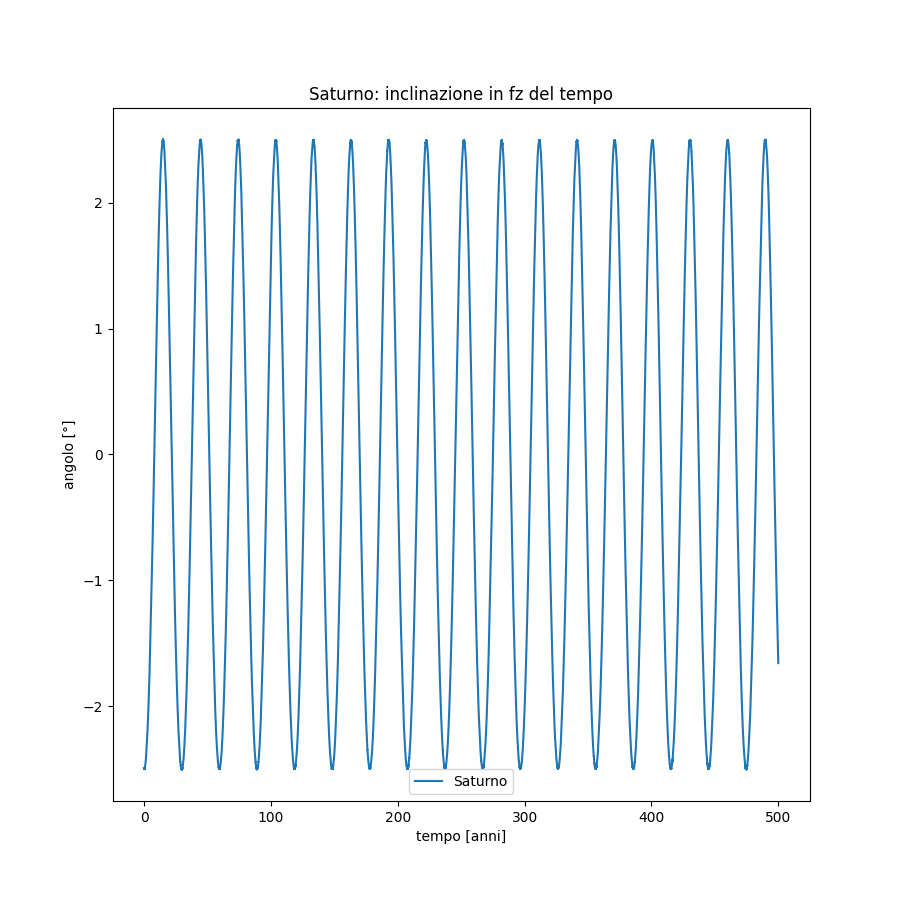
\includegraphics[width=5cm,height=3.75cm]{7_incli/sat_teta_tempo.png}\\
            \end{columns}
        \end{frame}